\documentclass[usenames,dvipsnames]{beamer}

% ---------------------------------------------------------

\usepackage[utf8]{inputenc}
\usepackage[T1]{fontenc}
\usepackage[english]{babel}

% ---------------------------------------------------------

\usepackage{appendixnumberbeamer}

\setbeamertemplate{navigation symbols}{}

\addtobeamertemplate{footline}{%
  \hspace*{\fill}%
  \llap{%
    \insertframenumber\,/\,\inserttotalframenumber%
    \hspace{5pt}%
  }
  \vskip4pt%
}

\AtBeginSection[]{
  \begin{frame}
    \tableofcontents[currentsection]
  \end{frame}
}

% ---------------------------------------------------------

\usepackage{graphicx}

% ---------------------------------------------------------

\usepackage{tikz}

\usetikzlibrary{graphs}
\usetikzlibrary{quotes}
\usetikzlibrary{calc}
\usetikzlibrary{arrows.meta}

\tikzset{
  node/.style= {draw, circle, inner sep=1.5},
  cnode/.style= {draw},
  root/.style= {fill=lightgray},
}

% ---------------------------------------------------------

\usepackage{macros}

% ---------------------------------------------------------

\title{
  Snapshottable stores
}
\author{
  \underline{Clément Allain} (INRIA Paris)\\
  Basile Clément (OCamlPro) \\
  Alexandre Moine (INRIA Paris) \\
  Gabriel Scherer (INRIA Paris)
}

% ---------------------------------------------------------
% ---------------------------------------------------------

\begin{document}

% ---------------------------------------------------------

\begin{frame}
\titlepage
\end{frame}

% ---------------------------------------------------------

\begin{frame}{From \OCaml to \Zoo}
\centering
\Huge
\begin{tabular}{ccccc}
      \raisebox{-.5\height}{\includegraphics[scale=0.3]{images/ocaml.png}}
    &&
      $\stackrel{\mbox{\Large\texttt{ocaml2zoo}}}{\longrightarrow}$
    &&
      \begin{tabular}{c}
          \includegraphics[scale=0.4]{images/coq.png}
        \\
          \textcolor{Green}{\Zoo}
        \\\\
          \includegraphics[scale=0.5]{images/iris.png}
      \end{tabular}
\end{tabular}
\end{frame}

% ---------------------------------------------------------

\begin{frame}{Specification: a simple store\dots}
\large
\[
  \iSpec{
    \iTrue
  }{
    \texttt{create ()}
  }{
    t
  }{
    \mathrm{store}\ t\ \emptyset
  }
\]
\vfill
\[
  \iSpec{
    \mathrm{store}\ t\ \sigma
  }{
    \texttt{ref}\ t\ v
  }{
    r
  }{
    r \notin \dom{\sigma} \iSep
    \mathrm{store}\ t\ \sigma[r \mapsto v]
  }
\]
\vfill
\[
  \begin{array}{cccc}
      \iSpec{
        \mathrm{store}\ t\ \sigma \iSep
        \sigma (r) = v
      }{
        \texttt{get}\ t\ r
      }{
        v
      }{
        \mathrm{store}\ t\ \sigma
      }
    &&&
      \iSpec{
        \mathrm{store}\ t\ \sigma \iSep
        r \in \dom{\sigma}
      }{
        \texttt{set}\ t\ r\ v
      }{
        v
      }{
        \mathrm{store}\ t\ \sigma[r \mapsto v]
      }
  \end{array}
\]
\end{frame}

\begin{frame}{\dots with persistent snapshots}
\Large
\[
  \iSpec{
    \mathrm{store}\ t\ \sigma
  }{
    \texttt{capture}\ t
  }{
    s
  }{
    \mathrm{store}\ t\ \sigma \iSep
    \mathrm{snapshot}\ t\ s\ \sigma
  }
\]
\vfill
\[
  \iSpec{
    \mathrm{store}\ t\ \sigma \iSep
    \mathrm{snapshot}\ t\ s\ \sigma'
  }{
    \texttt{restore}\ t\ s
  }{
    \texttt{()}
  }{
    \mathrm{store}\ t\ \sigma'
  }
\]
\end{frame}

% ---------------------------------------------------------

\begin{frame}{Implementation \emph{without} elision}
\centering
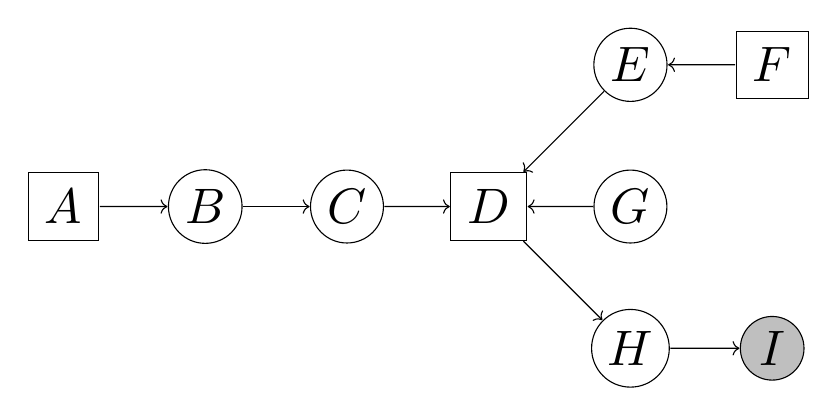
\begin{tikzpicture}[scale=1.8, every node/.style={transform shape}]
  \node [cnode] (a) at (0,0) {$A$} ;
  \node [node] (b) at (1,0) {$B$} ;
  \node [node] (c) at (2,0) {$C$} ;
  \node [cnode] (d) at (3,0) {$D$} ;
  \node [node] (e) at (4,1) {$E$} ;
  \node [cnode] (f) at (5,1) {$F$} ;
  \node [node] (g) at (4,0) {$G$} ;
  \node [node] (h) at (4,-1) {$H$} ;
  \node [node, root] (i) at (5,-1) {$I$} ;
  
  \graph {
    (a) -> (b) -> (c) -> (d) -> (h) -> (i) ;
    (d) <- (e) <- (f) ;
    (d) <- (g) ;
  } ;
\end{tikzpicture}
\end{frame}

% ---------------------------------------------------------

\begin{frame}{Rerooting \emph{without} elision}
\centering
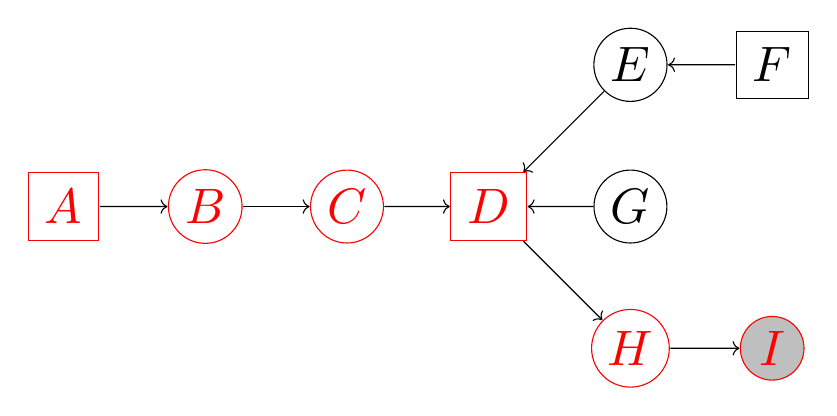
\begin{tikzpicture}[scale=1.8, every node/.style={transform shape}]
  \node [cnode, red] (a) at (0,0) {$A$} ;
  \node [node, red] (b) at (1,0) {$B$} ;
  \node [node, red] (c) at (2,0) {$C$} ;
  \node [cnode, red] (d) at (3,0) {$D$} ;
  \node [node] (e) at (4,1) {$E$} ;
  \node [cnode] (f) at (5,1) {$F$} ;
  \node [node] (g) at (4,0) {$G$} ;
  \node [node, red] (h) at (4,-1) {$H$} ;
  \node [node, red, root] (i) at (5,-1) {$I$} ;
  
  \graph {
    (a) -> (b) -> (c) -> (d) -> (h) -> (i) ;
    (d) <- (e) <- (f) ;
    (d) <- (g) ;
  } ;
\end{tikzpicture}
\end{frame}

% ---------------------------------------------------------

\begin{frame}{Rerooting \emph{without} elision}
\centering
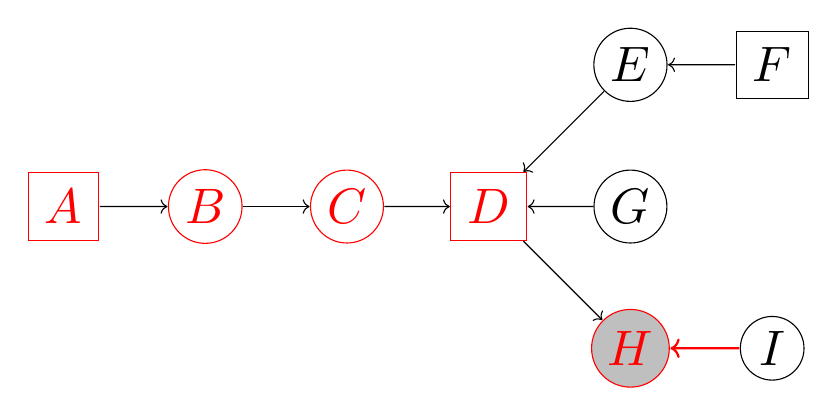
\begin{tikzpicture}[scale=1.8, every node/.style={transform shape}]
  \node [cnode, red] (a) at (0,0) {$A$} ;
  \node [node, red] (b) at (1,0) {$B$} ;
  \node [node, red] (c) at (2,0) {$C$} ;
  \node [cnode, red] (d) at (3,0) {$D$} ;
  \node [node] (e) at (4,1) {$E$} ;
  \node [cnode] (f) at (5,1) {$F$} ;
  \node [node] (g) at (4,0) {$G$} ;
  \node [node, red, root] (h) at (4,-1) {$H$} ;
  \node [node] (i) at (5,-1) {$I$} ;
  
  \graph {
    (a) -> (b) -> (c) -> (d) -> (h) <-[red,thick] (i) ;
    (d) <- (e) <- (f) ;
    (d) <- (g) ;
  } ;
\end{tikzpicture}
\end{frame}

% ---------------------------------------------------------

\begin{frame}{Rerooting \emph{without} elision}
\centering
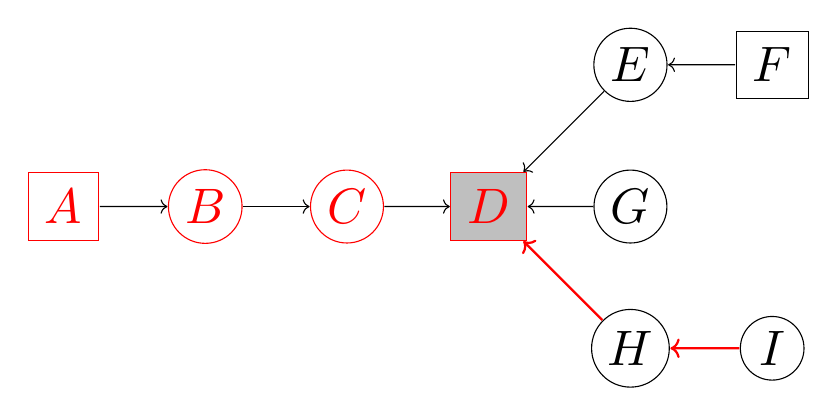
\begin{tikzpicture}[scale=1.8, every node/.style={transform shape}]
  \node [cnode, red] (a) at (0,0) {$A$} ;
  \node [node, red] (b) at (1,0) {$B$} ;
  \node [node, red] (c) at (2,0) {$C$} ;
  \node [cnode, red, root] (d) at (3,0) {$D$} ;
  \node [node] (e) at (4,1) {$E$} ;
  \node [cnode] (f) at (5,1) {$F$} ;
  \node [node] (g) at (4,0) {$G$} ;
  \node [node] (h) at (4,-1) {$H$} ;
  \node [node] (i) at (5,-1) {$I$} ;
  
  \graph {
    (a) -> (b) -> (c) -> (d) ;
    { [edges={red,thick}] (d) <- (h) <- (i) } ;
    (d) <- (e) <- (f) ;
    (d) <- (g) ;
  } ;
\end{tikzpicture}
\end{frame}

% ---------------------------------------------------------

\begin{frame}{Rerooting \emph{without} elision}
\centering
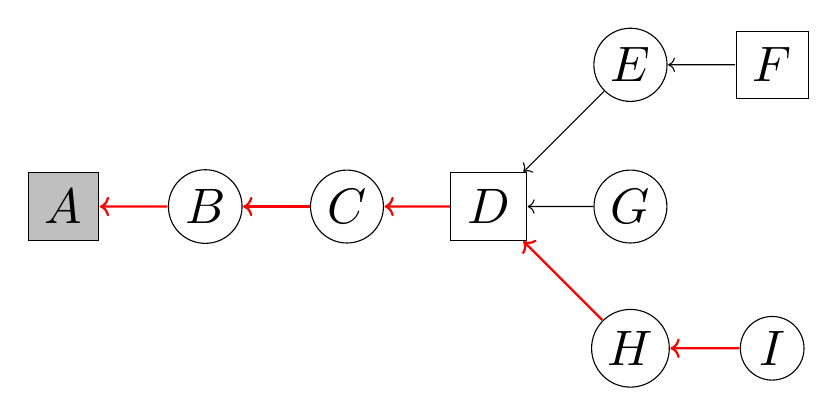
\begin{tikzpicture}[scale=1.8, every node/.style={transform shape}]
  \node [cnode, root] (a) at (0,0) {$A$} ;
  \node [node] (b) at (1,0) {$B$} ;
  \node [node] (c) at (2,0) {$C$} ;
  \node [cnode] (d) at (3,0) {$D$} ;
  \node [node] (e) at (4,1) {$E$} ;
  \node [cnode] (f) at (5,1) {$F$} ;
  \node [node] (g) at (4,0) {$G$} ;
  \node [node] (h) at (4,-1) {$H$} ;
  \node [node] (i) at (5,-1) {$I$} ;
  
  \graph {
    { [edges={red,thick}] (a) <- (b) <- (c) <- (d) <- (h) <- (i) } ;
    (d) <- (e) <- (f) ;
    (d) <- (g) ;
  } ;
\end{tikzpicture}
\end{frame}

% ---------------------------------------------------------

\begin{frame}{Historical tree \& generations}
\centering
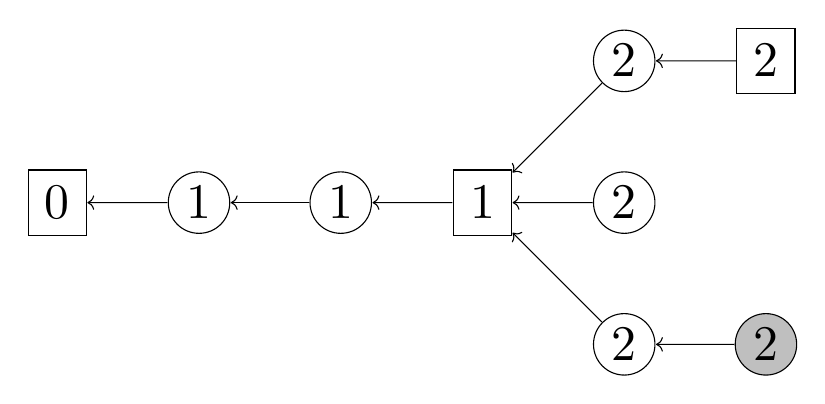
\begin{tikzpicture}[scale=1.8, every node/.style={transform shape}]
  \node [cnode] (a) at (0,0) {$0$} ;
  \node [node] (b) at (1,0) {$1$} ;
  \node [node] (c) at (2,0) {$1$} ;
  \node [cnode] (d) at (3,0) {$1$} ;
  \node [node] (e) at (4,1) {$2$} ;
  \node [cnode] (f) at (5,1) {$2$} ;
  \node [node] (g) at (4,0) {$2$} ;
  \node [node] (h) at (4,-1) {$2$} ;
  \node [node, root] (i) at (5,-1) {$2$} ;
  
  \graph {
    (a) <- (b) <- (c) <- (d) <- (h) <- (i) ;
    (d) <- (e) <- (f) ;
    (d) <- (g) ;
  } ;
\end{tikzpicture}
\end{frame}

% ---------------------------------------------------------

\begin{frame}{Implementation \emph{with} elision}
\centering
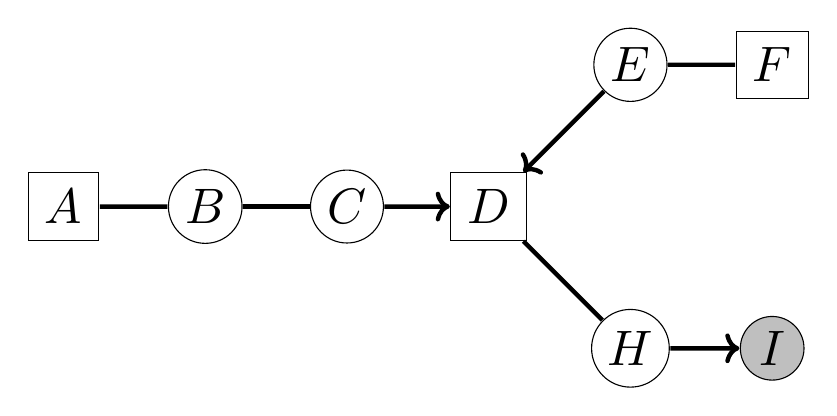
\begin{tikzpicture}[scale=1.8, every node/.style={transform shape}]
  \node [cnode] (a) at (0,0) {$A$} ;
  \node [node] (b) at (1,0) {$B$} ;
  \node [node] (c) at (2,0) {$C$} ;
  \node [cnode] (d) at (3,0) {$D$} ;
  \node [node] (e) at (4,1) {$E$} ;
  \node [cnode] (f) at (5,1) {$F$} ;
  \node [node] (h) at (4,-1) {$H$} ;
  \node [node, root] (i) at (5,-1) {$I$} ;
  
  \graph [edges=ultra thick] {
    (a) -- (b) -- (c) -> (d) -- (h) -> (i) ;
    (d) <- (e) -- (f) ;
  } ;
\end{tikzpicture}
\end{frame}

% ---------------------------------------------------------

\begin{frame}{Rerooting \emph{with} elision}
\centering
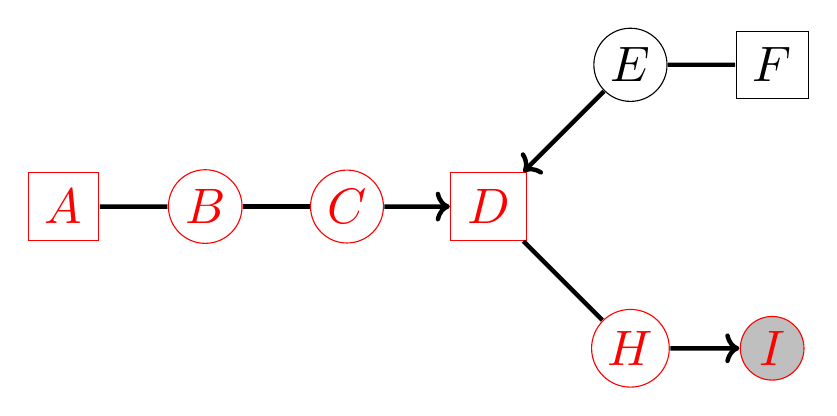
\begin{tikzpicture}[scale=1.8, every node/.style={transform shape}]
  \node [cnode, red] (a) at (0,0) {$A$} ;
  \node [node, red] (b) at (1,0) {$B$} ;
  \node [node, red] (c) at (2,0) {$C$} ;
  \node [cnode, red] (d) at (3,0) {$D$} ;
  \node [node] (e) at (4,1) {$E$} ;
  \node [cnode] (f) at (5,1) {$F$} ;
  \node [node, red] (h) at (4,-1) {$H$} ;
  \node [node, red, root] (i) at (5,-1) {$I$} ;
  
  \graph [edges=ultra thick] {
    (a) -- (b) -- (c) -> (d) -- (h) -> (i) ;
    (d) <- (e) -- (f) ;
  } ;
\end{tikzpicture}
\end{frame}

% ---------------------------------------------------------

\begin{frame}{Rerooting \emph{with} elision}
\centering
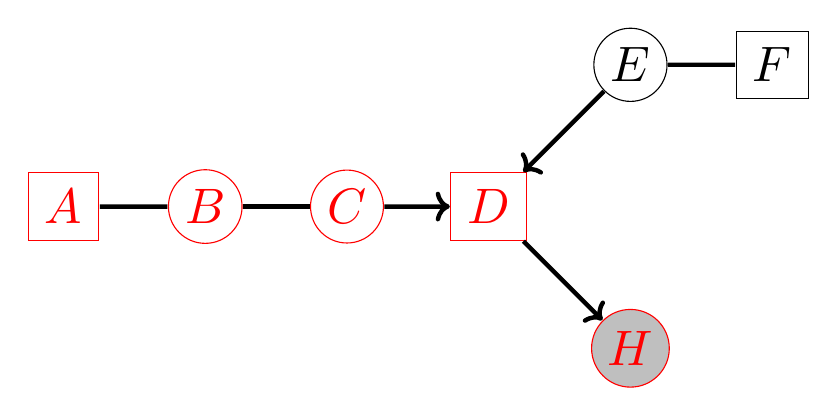
\begin{tikzpicture}[scale=1.8, every node/.style={transform shape}]
  \node [cnode, red] (a) at (0,0) {$A$} ;
  \node [node, red] (b) at (1,0) {$B$} ;
  \node [node, red] (c) at (2,0) {$C$} ;
  \node [cnode, red] (d) at (3,0) {$D$} ;
  \node [node] (e) at (4,1) {$E$} ;
  \node [cnode] (f) at (5,1) {$F$} ;
  \node [node, red, root] (h) at (4,-1) {$H$} ;
  
  \graph [edges=ultra thick] {
    (a) -- (b) -- (c) -> (d) -> (h) ;
    (d) <- (e) -- (f) ;
  } ;
\end{tikzpicture}
\end{frame}

% ---------------------------------------------------------

\begin{frame}{Rerooting \emph{with} elision}
\centering
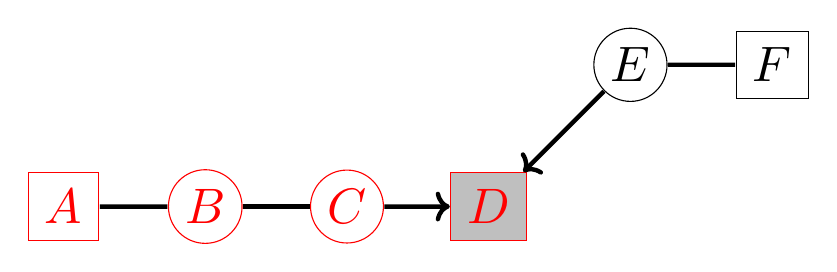
\begin{tikzpicture}[scale=1.8, every node/.style={transform shape}]
  \node [cnode, red] (a) at (0,0) {$A$} ;
  \node [node, red] (b) at (1,0) {$B$} ;
  \node [node, red] (c) at (2,0) {$C$} ;
  \node [cnode, red, root] (d) at (3,0) {$D$} ;
  \node [node] (e) at (4,1) {$E$} ;
  \node [cnode] (f) at (5,1) {$F$} ;
  
  \graph [edges=ultra thick] {
    (a) -- (b) -- (c) -> (d) ;
    (d) <- (e) -- (f) ;
  } ;
\end{tikzpicture}
\end{frame}

% ---------------------------------------------------------

\begin{frame}{Rerooting \emph{with} elision}
\centering
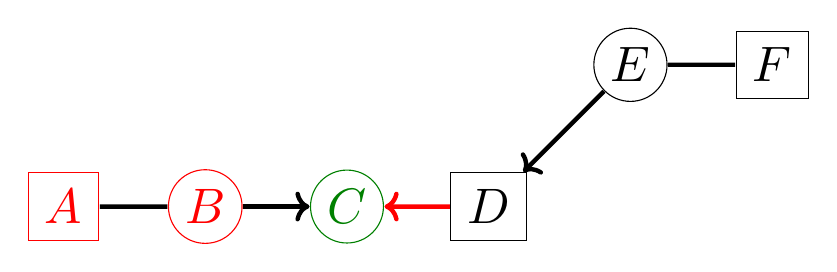
\begin{tikzpicture}[scale=1.8, every node/.style={transform shape}]
  \node [cnode, red] (a) at (0,0) {$A$} ;
  \node [node, red] (b) at (1,0) {$B$} ;
  \node [node, Green] (c) at (2,0) {$C$} ;
  \node [cnode] (d) at (3,0) {$D$} ;
  \node [node] (e) at (4,1) {$E$} ;
  \node [cnode] (f) at (5,1) {$F$} ;
  
  \graph [edges=ultra thick] {
    (a) -- (b) -> (c) <-[red] (d) ;
    (d) <- (e) -- (f) ;
  } ;
\end{tikzpicture}
\end{frame}

% ---------------------------------------------------------

\begin{frame}{Rerooting \emph{with} elision}
\centering
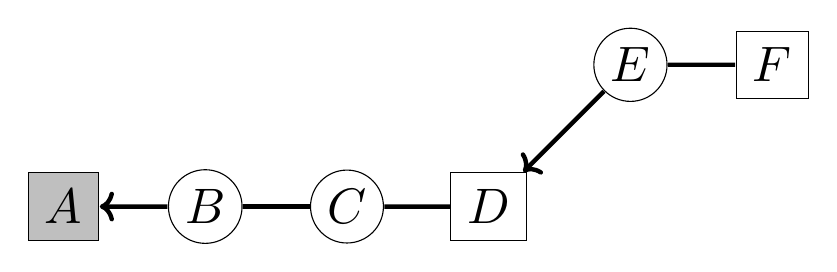
\begin{tikzpicture}[scale=1.8, every node/.style={transform shape}]
  \node [cnode, root] (a) at (0,0) {$A$} ;
  \node [node] (b) at (1,0) {$B$} ;
  \node [node] (c) at (2,0) {$C$} ;
  \node [cnode] (d) at (3,0) {$D$} ;
  \node [node] (e) at (4,1) {$E$} ;
  \node [cnode] (f) at (5,1) {$F$} ;
  
  \graph [edges=ultra thick] {
    (a) <- (b) -- (c) -- (d) ;
    (d) <- (e) -- (f) ;
  } ;
\end{tikzpicture}
\end{frame}

% ---------------------------------------------------------

\begin{frame}[plain, noframenumbering]
\LARGE
\begin{center}
  Merci de votre attention!
\end{center}
\end{frame}

% ---------------------------------------------------------

\end{document}
